\documentclass[sigconf,anonymous]{acmart}
% Submission draft. Numbers come from research/paper_draft.md (the lab log); run directories are
% listed in Appendix F, not in the text.

\settopmatter{printacmref=false, printccs=false, printfolios=true}
\setcopyright{none}
\renewcommand\footnotetextcopyrightpermission[1]{}
\acmConference[Preprint]{Under review}{2026}{}
\acmYear{2026}

\usepackage{booktabs}
\usepackage{multirow}
\usepackage{algorithm}
\usepackage{algpseudocode}
\usepackage{tikz}
\usetikzlibrary{arrows.meta,positioning,fit,calc,backgrounds}
\graphicspath{{figures/}}
\emergencystretch=1em

\newcommand{\lp}{\ell}
\newcommand{\nl}{\texttt{\textbackslash n}}
\newcommand{\U}{U}
\newcommand{\ci}[2]{\,[#1,\,#2]}
\newcommand{\Hr}[1]{HR@#1}
\newcommand{\Nd}[1]{NDCG@#1}
\newtheorem{proposition}{Proposition}

\begin{document}

\title{Beam Search Is Optional: Certified, Late-Entry Decoding for LLM Generative Recommenders}

\author{Anonymous Author(s)}
\affiliation{\institution{Anonymous Institution}\country{}}

\begin{abstract}
LLM-based generative recommenders emit an item as a short sequence of semantic-ID (SID) tokens and are
served with constrained beam search. Beam search costs one sequential forward pass per token and does not
guarantee that it returns the model's best items. We show that for catalog-sized tries it can be replaced
by \emph{certified exact decoding}. Every scored term is a log-probability $\le 0$, so one tree-attention
forward over the prompt and every first-level trie node bounds every item. A second forward scores the
best-bounded prefixes exactly, and an on-device test certifies that the returned top-$K$ is the global optimum
of the model's objective. Under trie normalization the bounds are two-sided, so the prefixes that guarantee
the certificate are known after the first forward. We also find that deeper SID codes do not need the lower
layers: prefix rows can enter the second forward at layer 26 of 28 through a small, label-free bridge from
their parent's state, without loss. Exact search also makes \emph{objective fusion} exact: an additive
per-item term, such as a collaborative model's score, keeps the certificate. On MiniOneRec (Qwen2-1.5B), a
certified top-10 takes 2.57\,ms on an H100. On the same GPU and prompts, FlashRec, a public SID serving
engine, takes 11.5\,ms and serves 5.4--6.4$\times$ fewer users per second. Fusing a 1-minute SASRec model into
the certified search raises HR@10 by 1.11 points, to 0.1825, at 2.83\,ms per request.
\end{abstract}

\keywords{generative recommendation, semantic IDs, constrained decoding, exact search, LLM inference}

\maketitle

% =====================================================================================================
\section{Introduction}

Generative retrieval with semantic IDs now serves production traffic~\cite{ax2506.13695,ax2602.22732,
ax2608.00938,ax2504.10507,spotify2026}. A recommender LLM reads the user's history and generates the next
item as a short code $\langle a,b,c\rangle$ from a hierarchical tokenizer~\cite{rajput2023}. A catalog trie
constrains decoding to codes that exist, and constrained beam search returns a ranked list. Serving cost
limits where these models can be used. The open serving engines therefore optimize beam search: they share
the prompt's key--value cache across beams, capture decode loops in CUDA graphs, and move trie masking onto
the GPU~\cite{flashrec,nvidiasidgr,ax2512.11529,ax2602.22647}.

We ask a different question: \emph{is beam search needed at all?} Its cost has a simple structure. A
three-level SID needs one forward for the prompt and one for each generated token, and at batch size 1 every
forward streams all the weights. So the number of sequential forwards sets the floor, not the beam width.
Beam search is also approximate. Under MiniOneRec's training objective, beam-50 recovers only 49\% of the exact
top-50 (Appendix~\ref{app:objective}).

Our observation is that the catalog trie is small compared with what one forward can process. The released
Office catalog has 88 first codes and 2,488 two-code prefixes. Every scored term is a log-probability, which
is $\le 0$, so the score of a prefix bounds the score of every item below it. One \emph{tree-attention} forward
over the prompt and all 88 first-level nodes therefore yields a bound for every item in the catalog. A second
forward over the most promising prefixes scores their items exactly. The returned top-$K$ is provably optimal
as soon as the $K$-th exact score beats every remaining bound. This check runs on the device, in the same
CUDA graph, for every request. Certification is classical in exact search for
sequence models~\cite{stahlberg2019,stahlberg2022,fagin2003} and was recently stated for generative
recommendation as a post-hoc completion of beam search~\cite{ax2609.33745}. We make it the decoder and show
what makes it cheap.

\paragraph{Contributions.}
\begin{itemize}
\item \textbf{Certified exact decoding} (\S\ref{sec:certified}). A fixed-shape, two-forward decoder returns a
  per-request optimality certificate and certifies 100\% of requests, with no violations against brute force.
  Under trie normalization the bounds are \emph{two-sided}. The set of prefixes that guarantees the certificate
  is therefore known after the first forward. It averages at most $1.1K$ prefixes and is within 1.2--2.1$\times$
  of the instance-optimal set. On synthetic catalogs of up to 1M SIDs, the required expansion stays flat.
\item \textbf{Late entry} (\S\ref{sec:late}). A child row's state at layer $e$ is predicted from its parent's
  state at the same depth, using a small bridge distilled from the frozen model without labels. The third code
  then needs only the top 2 of 28 layers, and the first-level rows only the top 10, with no measurable quality
  loss.
\item \textbf{Exact objective fusion} (\S\ref{sec:fusion}). Any additive item term keeps the certificate,
  including priors, bids, eligibility filters and collaborative scores. Beam-then-rerank cannot change which
  items are retrieved; fused certified search can.
\item \textbf{Evaluation} (\S\ref{sec:experiments}). On the same H100 and prompts, certified decoding is
  4.5$\times$ faster per request than FlashRec~\cite{flashrec} and serves 5.4--6.4$\times$ more users per
  second. Both engines run beam search at the same throughput, so the gain comes from the decoder. Results
  hold on two datasets and on 3B and 7B backbones.
\end{itemize}

\begin{figure}[t]
\centering
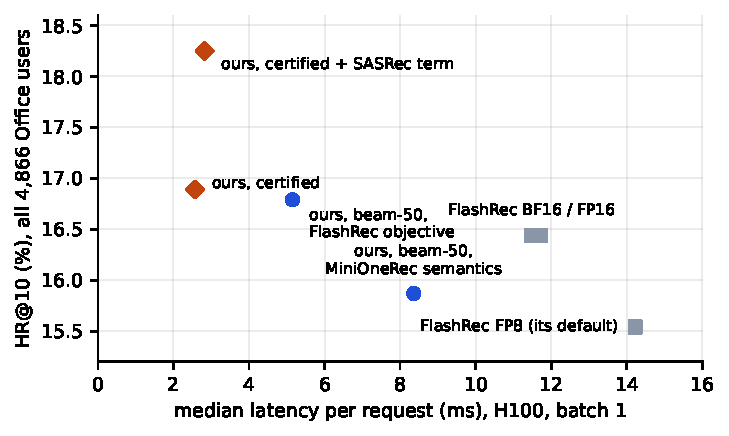
\includegraphics[width=\linewidth]{h100_latency_quality.pdf}
\vspace{-6mm}
\caption{Latency and quality on one H100: Office dataset, batch 1, all engines in the same allocation.
FlashRec is a public SID serving engine run on our prompts and catalog (FP16 coincides with BF16). HR@10 is
over all 4,866 test users (certified points: same configurations, other runs).}
\label{fig:headline}
\vspace{-2mm}
\end{figure}

% =====================================================================================================
\section{Setting}
\label{sec:setting}

\paragraph{Model and data.} We use MiniOneRec~\cite{ax2510.24431}, an open reproduction of OneRec-style
generative recommendation. It is Qwen2-1.5B~\cite{ax2407.10671} (28 layers, $d=1536$, 12 query and 2 key--value
heads) fine-tuned on Amazon \emph{Office Products} and \emph{Industrial and Scientific}. Items carry a
three-level code $\langle a,b,c\rangle$ from an RQ-VAE with 256 codes per level, appended to the vocabulary as
600 tokens. The Office catalog has 3,459 items (3,444 distinct SIDs), 88 first codes and 2,488 two-code
prefixes; Industrial has 48 first codes. Prompts are 76--121 tokens long and share a 69-token instruction
prefix. The test splits contain 4,866 (Office) and 4,533 (Industrial) users.

\paragraph{Scores.} For a prompt $x$ and item $i=\langle a,b,c\rangle$ we write
\begin{equation}
s(i) = \lp(a) + w_b\,\lp(b\mid a) + w_c\,\lp(c\mid a,b) + w_s\,\lp(\nl,\mathrm{EOS}\mid a,b,c),
\label{eq:score}
\end{equation}
where each $\lp$ is a log-probability under one of three \emph{normalizations}. \emph{Full}: log-softmax over the
whole vocabulary, which is MiniOneRec's training objective. \emph{Codebook}: log-softmax over the 256 codes of
that level, as in FlashRec. \emph{Trie}: log-softmax over the valid children of the current prefix. MiniOneRec
decodes with beam width 50, full normalization, $w=(1,1,1)$, and scores a forced newline and EOS after $c$. Our
default, \emph{cbtrie}, uses codebook normalization for $a$ and $b$, trie normalization for $c$, and
$w=(1,0.75,0)$. These weights were chosen on the validation split. Every term in Eq.~\ref{eq:score} is $\le 0$,
the property all our bounds rely on.

\paragraph{Metrics.} SID-level HR@$K$ and NDCG@$K$ on all test users. Every quality difference is paired over
users, with 95\% bootstrap intervals from 2,000 resamples, written $\Delta\,[\text{lo},\text{hi}]$ in points.
Latency is measured at batch 1 on a frozen cohort of 500 test users, $2\times500$ requests, CUDA-synchronized,
excluding compilation and graph capture. We report the median. Absolute latency varies by up to 10\% between
allocations of the same GPU type, so every comparison we draw a conclusion from runs within one allocation.

% =====================================================================================================
\section{Certified exact decoding}
\label{sec:certified}

\begin{figure}[t]
\centering
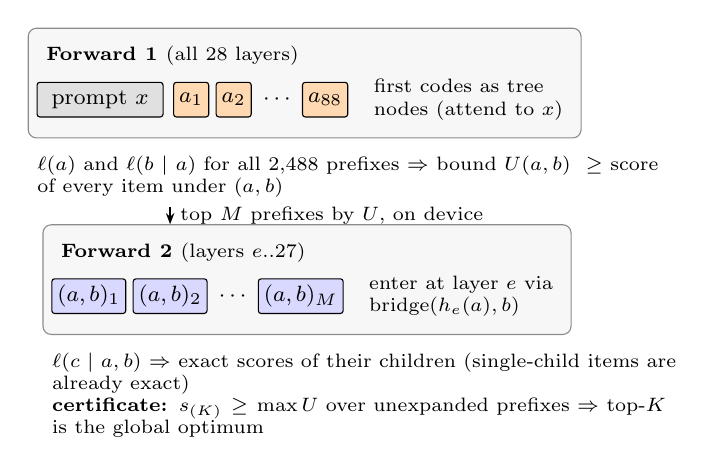
\begin{tikzpicture}[
  font=\footnotesize, >={Stealth[length=4pt]},
  tok/.style={draw, rounded corners=1pt, minimum height=4.4mm, inner sep=2pt},
  stage/.style={draw=black!45, rounded corners=3pt, inner sep=3pt, fill=black!3},
  lab/.style={font=\scriptsize, align=left, text width=80mm}]
  % ---- forward 1
  \node[tok, minimum width=16mm, fill=black!12] (x) {prompt $x$};
  \node[tok, right=1.2mm of x, fill=orange!30] (a1) {$a_1$};
  \node[tok, right=0.8mm of a1, fill=orange!30] (a2) {$a_2$};
  \node[right=0.2mm of a2] (ad) {$\cdots$};
  \node[tok, right=0.2mm of ad, fill=orange!30] (an) {$a_{88}$};
  \node[font=\scriptsize, right=2mm of an, align=left] (n1) {first codes as tree\\nodes (attend to $x$)};
  \node[font=\scriptsize\bfseries, above=0.8mm of x.north west, anchor=south west] (t1) {Forward 1 \textmd{(all 28 layers)}};
  \begin{scope}[on background layer]\node[stage, fit=(t1)(x)(an)(n1)] (f1) {};\end{scope}
  \node[lab, below=1mm of f1.south west, anchor=north west] (b1)
    {$\lp(a)$ and $\lp(b\mid a)$ for all 2,488 prefixes $\Rightarrow$ bound $\U(a,b)\ \ge$ score of every item under $(a,b)$};
  % ---- forward 2
  \node[tok, below=9mm of b1.south west, anchor=north west, xshift=3mm, fill=blue!15] (p1) {$(a,b)_1$};
  \node[tok, right=0.8mm of p1, fill=blue!15] (p2) {$(a,b)_2$};
  \node[right=0.2mm of p2] (pd) {$\cdots$};
  \node[tok, right=0.2mm of pd, fill=blue!15] (pm) {$(a,b)_M$};
  \node[font=\scriptsize, right=2mm of pm, align=left] (n2) {enter at layer $e$ via\\bridge$(h_e(a),b)$};
  \node[font=\scriptsize\bfseries, above=0.8mm of p1.north west, anchor=south west] (t2) {Forward 2 \textmd{(layers $e$..27)}};
  \begin{scope}[on background layer]\node[stage, fit=(t2)(p1)(pm)(n2)] (f2) {};\end{scope}
  \draw[->, thick] (b1.south -| p2.north) ++(0,0) -- node[font=\scriptsize, right]{top $M$ prefixes by $\U$, on device} (f2.north -| p2.north);
  \node[lab, below=1mm of f2.south west, anchor=north west] (b2)
    {$\lp(c\mid a,b)$ $\Rightarrow$ exact scores of their children (single-child items are already exact)\\
     \textbf{certificate:} $s_{(K)} \ge \max\U$ over unexpanded prefixes $\Rightarrow$ top-$K$ is the global optimum};
\end{tikzpicture}
\vspace{-2mm}
\caption{Certified decoding of one request. Both forwards have fixed shapes, so a request is one CUDA-graph
replay.}
\label{fig:overview}
\vspace{-3mm}
\end{figure}

\subsection{Bounds and the certificate}
Let $p=(a,b)$ be a two-code prefix and $\U(p)=\lp(a)+w_b\,\lp(b\mid a)$. Since $w_c\lp(c\mid a,b)\le0$ and
$w_s\lp(\cdot)\le0$, every item under $p$ scores at most $\U(p)$. Forward~1 appends every first code
$a\in A$ to the prompt as a \emph{tree node}: node $a$ attends to the prompt and to itself, at the position the
first SID token would occupy. One forward thus yields $\lp(a)$ for all $a$ and $\lp(b\mid a)$ for every valid
$(a,b)$, which is $\U$ for the whole trie (Fig.~\ref{fig:overview}). Forward~2 feeds the token $b$ for the $M$
prefixes with the largest $\U$, reusing the K/V of their parent nodes, and yields exact scores for all their
children. (If the forced suffix is scored, a third forward over the $N$ best items adds $\lp(\nl,\mathrm{EOS})$;
our default sets $w_s=0$.) Algorithm~\ref{alg:certified} returns the pool sorted by exact score with a per-$K$
certificate.

\begin{proposition}[Soundness]\label{prop:sound}
If the $K$-th largest exact score in the pool is at least $\U(p)$ for every unexpanded prefix $p$, the pool's
top $K$ is the global top $K$ of Eq.~\ref{eq:score}.
\end{proposition}

This is the stopping rule of exact $n$-best search~\cite{stahlberg2022} and of Fagin's threshold
algorithm~\cite{fagin2003}. What makes it cheap here is that all bounds come from a single forward.

\begin{algorithm}[t]
\caption{Certified exact top-$K$ (one request)}
\label{alg:certified}
\small
\begin{algorithmic}[1]
\Require prompt $x$; trie with first codes $A$; budget $M$
\State $\lp(a),\ \lp(b\mid a)\ \forall (a,b)$ $\gets$ \textsc{Forward}$\big([x;\,A \text{ as tree nodes}]\big)$
\State $\U(a,b) \gets \lp(a) + w_b\,\lp(b\mid a)$ \Comment{$\ge$ every item under $(a,b)$}
\State $P \gets$ the $M$ multi-child prefixes with the largest $\U$
\State $\lp(c\mid a,b)\ \forall (a,b)\in P$ $\gets$ \textsc{Forward}$\big(P\big)$, from layer $e$ \Comment{\S\ref{sec:late}}
\State pool $\gets$ children of $P$ $\cup$ items under single-child prefixes, with exact scores
\State $\tau \gets \max\{\U(p) : p \notin P,\ p \text{ multi-child}\}$
\State \Return pool sorted by score; certified$_K \gets [\,s_{(K)} \ge \tau\,]$ for each $K$
\end{algorithmic}
\end{algorithm}

\subsection{Trie normalization makes the bound tight and two-sided}
Under trie normalization, $\lp(c\mid a,b)$ is a log-softmax over the $n_p$ valid children of $p$. Two
consequences follow. First, a prefix with one child has $\lp(c\mid a,b)=0$, so its item is scored exactly by
Forward~1. On Office, 1,907 of the 2,488 prefixes have a single child, so Forward~2 only needs the 581
multi-child prefixes. Second, the best child of $p$ has log-probability at least $-\log n_p$, so some item under
$p$ scores at least $L(p)=\U(p)-w_c\log n_p$. The bound is two-sided.

\begin{proposition}[Instance optimality]\label{prop:necessary}
Let $\tau^*$ be the true $K$-th score. Any decoder whose only information about an unexpanded prefix is $\U(p)$
must expand every multi-child $p$ with $\U(p)>\tau^*$: its children's log-softmax could put almost all mass on
one child scoring above $\tau^*$. Best-first expansion by $\U$ attains this minimal set $N$.
\end{proposition}

\begin{proposition}[Guaranteed expansion set]\label{prop:guaranteed}
Let $\tau_L$ be the $K$-th largest value among the exact single-child scores and $\{L(p)\}$ over multi-child
prefixes. Expanding $E=\{p : \U(p)\ge\tau_L\}\supseteq N$ always certifies the top $K$, and $|E|$ is known
right after Forward~1.
\end{proposition}

Proofs are in Appendix~\ref{app:proofs}. Codebook or full normalization admits no lower bound, because the
valid children can hold arbitrarily little probability mass. Proposition~\ref{prop:guaranteed} turns the budget
$M$ into a choice the server can check before Forward~2: if $|E|>M$, the request is detected after Forward~1
and can be re-run with a larger budget.

\subsection{Late entry: deeper codes skip the lower layers}
\label{sec:late}
The logit lens shows that SID codes are decided in the last 6--9 layers. Early exit, which runs only the
\emph{first} $k$ layers for the third code, keeps HR@10 but loses 2.4--3.7 points of HR@1
(\S\ref{sec:exp-late}). We instead let each prefix row of Forward~2 \emph{enter late}. A row $(a,b)$ starts at
layer $e$ with an input built from its parent node's residual stream $h_e(a)$, which Forward~1 has already
computed, and runs layers $e,\dots,27$ with exact attention to the prompt and the parent's K/V:
\begin{equation}
\begin{split}
x_e(a,b) = h_e(a) &+ R_e\,\bigl[h_e(a);E_b;E_a;1\bigr]\\
 &+ \mathrm{MLP}_e\bigl([\mathrm{rms}(h_e(a));E_b;E_a]\bigr).
\end{split}
\label{eq:bridge}
\end{equation}
Here $E$ is the token embedding and $R_e$ is a ridge regression fit without labels. The MLP has 2,048 hidden
units and a zero-initialized output, about 10M parameters per entry layer. It is distilled from the frozen
model: we minimize the KL divergence between the full-depth and the late-entry distributions of the third code
on MiniOneRec's \emph{validation} prompts. Half of each row's weight is uniform and half follows a softmax of
its bound $\U$, which emphasizes the rows that decide the ranking. Training takes 1--2 minutes on one H100 and
uses no item labels.

The same construction applies to Forward~1. The 88 first-code rows enter at layer 18, bridged from the last
prompt token. Since SID nodes are always the last positions, no later token ever needs a bridged row's K/V below
its entry layer. The certificate then holds for the bridged objective, and we measure quality against the
full-depth model.

\subsection{Exact objective fusion}
\label{sec:fusion}
Production rankers rarely serve the model's log-probability alone. They add item terms such as priors, bids,
freshness, eligibility, or a collaborative model's opinion. Beam search can apply such a term only after it has
pruned. Certified search handles any additive term $v_u(i)$ exactly. The bound becomes
$\U(p)+\max_{i\in p}v_u(i)$, a scatter-max per request; Forward~2 still has $M$ rows, and
Proposition~\ref{prop:sound} is unchanged. A filter is a term in $\{0,-\infty\}$: a prefix whose items are all
ineligible is never expanded. We use a SASRec model~\cite{kang2018} (2 layers, $d=64$, 58\,s of training) with
$v_u(i)=\beta\log q_{\text{SASRec}}(i\mid\text{history})$ and $\beta=0.5$ chosen on validation. SASRec runs
inside the same CUDA graph on a side stream, so a request carries only the user's 20-item history.

\subsection{Engine}
\label{sec:engine}
All decoders, including our beam-search baselines, run in one hand-written engine. Each request is a single
CUDA-graph replay of a Qwen2 forward written from the safetensors weights. The engine fuses the QKV and gate/up
projections, uses FP16 with a pre-scaled query, and computes the shared prompt's K/V once and keeps it cached.
A Triton kernel computes shared-prefix attention for tree and beam rows, with one program per (user, row, KV
head). Appendix~\ref{app:engine} gives the engine's latency ladder from Hugging Face \texttt{generate}
(869\,ms on an A6000) down to 2.75\,ms on an H100.

% =====================================================================================================
\section{Experiments}
\label{sec:experiments}

We answer five questions. \textbf{RQ1}: How fast is certified decoding compared with beam search and with a
public SID serving engine? \textbf{RQ2}: How does it change quality, and what does exact fusion add?
\textbf{RQ3}: What does the certificate cost as $K$ and the catalog grow? \textbf{RQ4}: Is late entry lossless?
\textbf{RQ5}: Do the results transfer to other backbones?

\paragraph{Baselines.} (i) MiniOneRec's own beam search (width 50, full normalization, forced suffix) in our
engine, so the decoder is the only difference. (ii) Beam-50 under FlashRec's objective (per-level codebook
softmax, no suffix). (iii) FlashRec 0.1.2~\cite{flashrec}, an open SID-GR engine with CUDA-graph wide beam
search, a fused trie kernel, a restricted LM head, a radix prefix cache and FP8 by default. FlashRec supports
only Qwen3, so we added Qwen2 support (QKV bias, no QK-norm) with a 60-line patch. It decodes our exact token
ids and catalog. Its radix cache holds the shared 69-token prefix, as our template cache does, and all other
prefixes are evicted before each timed request. NVIDIA's SID-GR example~\cite{nvidiasidgr} could not be run: its
decode-attention kernel is a private submodule. (iv) Beam-then-rerank with the same SASRec term.

\subsection{RQ1: Speed}
\label{sec:exp-speed}

\begin{table}[t]
\caption{Same H100 allocation, Office, batch 1. Latency is the median over $2\times500$ requests; throughput
is users/s at the largest batch each decoder fits (B = 128; 64 for our beam-50). HR@10 is over all 4,866 test
users; for the two certified rows it comes from runs of the same configuration in other allocations.}
\label{tab:speed}
\vspace{-2mm}
\small
\setlength{\tabcolsep}{3.2pt}
\begin{tabular*}{\linewidth}{@{\extracolsep{\fill}}lrrrr@{}}
\toprule
decoder & ms & p95 & users/s & HR@10 \\
\midrule
FlashRec, BF16                         & 11.48 & 11.64 & --    & 0.1644 \\
FlashRec, FP16                         & 11.71 & 12.02 & 500   & 0.1644 \\
FlashRec, FP8 (default)                & 14.22 & 14.45 & 489   & 0.1554 \\
\midrule
ours, beam-50, MiniOneRec objective    & 8.36  & 9.04  & --    & 0.1587 \\
ours, beam-50, FlashRec objective      & 5.15  & 5.30  & 489   & 0.1679 \\
ours, certified                        & \textbf{2.57} & 2.65 & 2,681 & 0.1689 \\
\quad + dynamic FP8                    & --    & --    & \textbf{3,148} & -- \\
ours, certified + SASRec term          & 2.83  & 2.92  & --    & \textbf{0.1825} \\
\bottomrule
\end{tabular*}
\vspace{-3mm}
\end{table}

Table~\ref{tab:speed} and Fig.~\ref{fig:headline} compare all decoders in one allocation. Certified decoding
takes 2.57\,ms, 4.5$\times$ less than FlashRec and 3.3$\times$ less than MiniOneRec's beam search in our own
engine. The gap does not depend on where the timer stops. FlashRec's GPU kernels alone take 6.78\,ms per request
(1,878 kernels, profiled over 50 requests), more than our whole end-to-end time; the rest of its 11.7\,ms is
host-side scheduling. FP8, FlashRec's default, is slower than BF16 at batch 1 on this 1.5B model and costs
$-0.90\,[-1.32,-0.47]$ HR@10.

\emph{The engines are comparable; the decoders are not.} With beam-50, our engine and FlashRec serve the same
number of users per second (457--489 vs.\ 408--500 across batch sizes 16--128; Fig.~\ref{fig:throughput}).
Certified decoding serves 2,310--2,681 users/s in FP16 and up to 3,148 with dynamic per-token FP8, which is
quality-neutral. That is 5.4--6.4$\times$ FlashRec. It simply processes fewer rows per user: 88 tree nodes and
16 prefix rows, against 88 + 150 rows for beam-50 in the same engine.

Long candidate lists stay cheap. A certified top-500 takes 2.92\,ms, against 18.1\,ms for MiniOneRec's beam-500,
and serves 450 vs.\ 71 users/s. The second forward grows with the number of multi-child prefixes the certificate
needs (about $0.4K$), not with the beam width.

\begin{figure}[t]
\centering
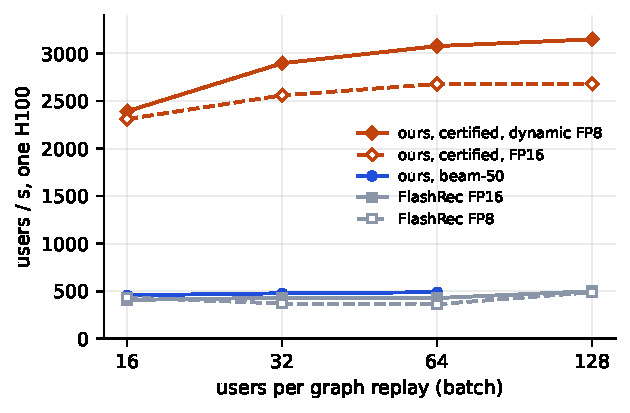
\includegraphics[width=0.92\linewidth]{flashrec_throughput.pdf}
\vspace{-3mm}
\caption{Throughput on one H100. With beam-50, both engines serve the same number of users; certified decoding
serves 5.4--6.4$\times$ more.}
\label{fig:throughput}
\vspace{-3mm}
\end{figure}

\subsection{RQ2: Quality and exact fusion}
\label{sec:exp-quality}

\begin{table}[t]
\caption{Quality on all test users (Office 4,866; Industrial 4,533). Fused vs.\ certified: HR@10
$+1.11\,[+0.62,+1.60]$ (Office), $+0.51\,[+0.07,+0.95]$ (Industrial). Fused vs.\ rerank: HR@10
$+0.25\,[+0.08,+0.43]$. Paired differences in points, 95\% bootstrap intervals.}
\label{tab:quality}
\vspace{-2mm}
\footnotesize
\setlength{\tabcolsep}{3pt}
\begin{tabular*}{\linewidth}{@{\extracolsep{\fill}}lrrrr@{}}
\toprule
decoder & HR@1 & HR@10 & NDCG@10 & HR@50 \\
\midrule
\multicolumn{5}{@{}l}{\emph{Office}} \\
MiniOneRec beam-50 (FP32)     & 0.0947 & 0.1589 & 0.1249 & 0.2370 \\
certified (cbtrie)            & 0.0993 & 0.1714 & 0.1319 & 0.2513 \\
certified, then SASRec rerank & 0.1021 & 0.1800 & 0.1377 & 0.2513 \\
certified + SASRec (fused)    & \textbf{0.1025} & \textbf{0.1825} & \textbf{0.1391} & \textbf{0.2721} \\
\midrule
\multicolumn{5}{@{}l}{\emph{Industrial}} \\
MiniOneRec beam-50            & -- & 0.1582 & -- & -- \\
certified (cbtrie)            & -- & 0.1617 & -- & -- \\
certified + SASRec (fused)    & -- & \textbf{0.1668} & -- & -- \\
\bottomrule
\end{tabular*}
\vspace{-3mm}
\end{table}

\paragraph{The decoder improves quality before fusion.} On Office, certified decoding with the cbtrie objective
reaches HR@10 0.1714, against 0.1589 for MiniOneRec's FP32 beam decode of the same checkpoint
(Table~\ref{tab:quality}). This gain comes from the scoring rule, not from exactness. Restricted
normalizations, which production engines adopt for speed, score better than the training objective even under
beam-50 (HR@10 0.1667 codebook, 0.1648 trie, vs.\ 0.1589 full), and the validation-tuned weight
$w_c=0.75$ discounts the third code, which carries a catalog-structure penalty unrelated to the user
(Appendix~\ref{app:objective}). On Industrial, no scoring rule significantly beats the original objective,
and certified decoding is at least as good as beam (Table~\ref{tab:quality}).

\paragraph{Fusion changes what is retrieved.} Adding $\beta\log q_{\text{SASRec}}$ inside the certified search
raises Office HR@10 by $+1.11$ points and beats reranking the same list by $+0.25$. That is $+2.36$ over MiniOneRec's own decode, with no LLM training, and
on par with the best \emph{trained} result we know of on this split (0.1834~\cite{ax2608.20611}). Reranking the
LLM's top-50 with the same term recovers most of the HR@10 gain. It cannot change the candidate set, so its HR@50
does not move (0.2513), while fusion adds 2.08 points. At $K=500$ fusion lifts HR@500 from 0.504 to 0.543 on
Office and from 0.523 to 0.544 on Industrial. Certification is unaffected: 100\% of Office users certify the
fused top-10. The fused top-500 needs $M=256$ on Office; on Industrial, $M=512$ (4.23\,ms) certifies all users.

\paragraph{Reranking fails when the term matters.} With a synthetic item value $\lambda v$, $v\sim\mathcal N(0,1)$,
reranking the LLM's top-50 recovers 99.2\% of the exact top-10 at $\lambda=0.5$ but only 50.0\% at $\lambda=2$.
Certified search stays exact. Filters behave the same way: when 5\% of items are eligible, filtering the LLM's
top-50 recovers only 30.5\% of the exact eligible top-10. Two certified forwards return it exactly, and
filter-after-retrieval needs a 10$\times$ longer list to catch up.

\paragraph{Against FlashRec.} Paired against FlashRec FP16, certified decoding gains $+0.45\,[+0.00,+0.90]$
HR@10 and the fused decoder gains $+1.81\,[+1.23,+2.36]$. Part of FlashRec's deficit is numerical. On our Qwen2
port, its first-code log-probabilities differ from the reference model by 0.23 nats on average. We could not
attribute this to any component we could isolate (Appendix~\ref{app:flashrec}). We therefore also compare with
our exact implementation of FlashRec's objective (HR@10 0.1679). Certified decoding matches it at half the
latency ($+0.10\,[-0.31,+0.58]$), and fusion adds $+1.46\,[+0.88,+2.01]$.

\subsection{RQ3: What the certificate costs}
\label{sec:exp-cost}

\begin{figure}[t]
\centering
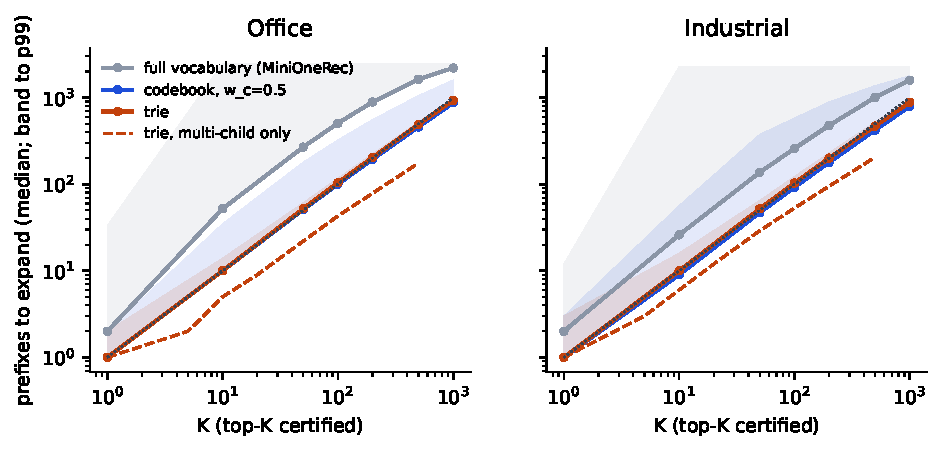
\includegraphics[width=\linewidth]{certificate_kscale.pdf}
\vspace{-6mm}
\caption{Prefixes the certificate must expand to prove the top $K$ (median; band to p99), from exhaustive FP32
scores of all test users. Under trie or codebook normalization the cost is about $K$; under the full-vocabulary
objective it approaches the whole trie.}
\label{fig:kscale}
\vspace{-3mm}
\end{figure}

\paragraph{The normalization decides whether exact search is affordable.} Fig.~\ref{fig:kscale} shows the
prefixes whose bound exceeds the $K$-th exact score, computed from exhaustive scores of every SID for every
test user. Under trie normalization, certifying the top-10 needs a median of 10 prefixes (p99: 14), and the top
1,000 needs 932. Under MiniOneRec's full-vocabulary objective, the top-10 needs 52 at the median and 1,715 at
p90 of the 2,488 prefixes. Probability that leaks off the codebook, together with the forced suffix, makes the
bound loose. Counting only multi-child prefixes, trie normalization needs a median of 5 for $K=10$ and 175 for
$K=500$.

\begin{table}[t]
\caption{Guaranteed expansion set $|E|$ (Prop.~\ref{prop:guaranteed}; mean / p99 / max) against the minimal set
$|N|$ (Prop.~\ref{prop:necessary}; mean / max), all test users.}
\label{tab:bounds}
\vspace{-2mm}
\small
\setlength{\tabcolsep}{3pt}
\begin{tabular*}{\linewidth}{@{\extracolsep{\fill}}rllll@{}}
\toprule
& \multicolumn{2}{c}{Office (late entry)} & \multicolumn{2}{c}{Industrial} \\
\cmidrule(lr){2-3}\cmidrule(lr){4-5}
$K$ & $|E|$ & $|N|$ & $|E|$ & $|N|$ \\
\midrule
1   & 0.8 / 4 / 8       & 0.6 / 3    & 1.0 / 5 / 9       & 0.7 / 4 \\
10  & 6.7 / 16 / 24     & 4.5 / 13   & 10.6 / 23 / 29    & 5.0 / 14 \\
50  & 29.7 / 50 / 62    & 21.7 / 43  & 41.5 / 62 / 75    & 25.1 / 45 \\
100 & 54.6 / 83 / 99    & 41.5 / 71  & 72.7 / 102 / 116  & 47.9 / 81 \\
500 & 203 / 248 / 267   & 166 / 220  & 259 / 318 / 342   & 188 / 256 \\
\bottomrule
\end{tabular*}
\vspace{-3mm}
\end{table}

\paragraph{The guaranteed set is small.} Table~\ref{tab:bounds} shows that the set known after Forward~1 averages
at most $1.1K$ prefixes at every $K$ ($0.41K$ at $K=500$) and is 1.2--2.1$\times$ the provable minimum. Our
$M=16$ configuration covers $|E|$ for 99\% of Office users and still certifies 100\% of them, because $E$
over-approximates $N$. Against brute-force FP32 scoring of all 3,444 SIDs, we found no certified request whose
top-$K$ was wrong.

\paragraph{Catalog size.} The released catalogs are small, but the model's codes address
$88\times256\times256=5.8$M SIDs. We densify the trie up to 1M SIDs, by adding siblings under real prefixes or
new prefixes under real first codes, and score real prompts with the real model (Fig.~\ref{fig:catalog}). Quality
has no meaning for synthetic items, but cost does. The minimal expansion is flat in catalog size, at
$|N|\approx8.4/42/410$ for $K=10/50/500$ from 10k to 1M SIDs, and so is latency at a fixed budget: 6.33\,ms on
the real catalog and 6.36\,ms at 1M SIDs (A6000, $M=16$). Forward~1 always carries the prompt and the 88 first
codes, and Forward~2 carries $M$ rows. Certified top-10 holds for at least 99.6\% of users at $M=16$ and for 100\%
at $M=32$, at every size. Industrial replicates this ($|N|\approx7.8/38/350$). The two-sided guarantee does
\emph{not} scale: $|E|$ grows with branching as the $-\log n_p$ lower bound loosens. On dense tries, Forward~2
should therefore be sized by a fixed $M$, with a fallback for the rare uncertified request.

\begin{figure}[t]
\centering
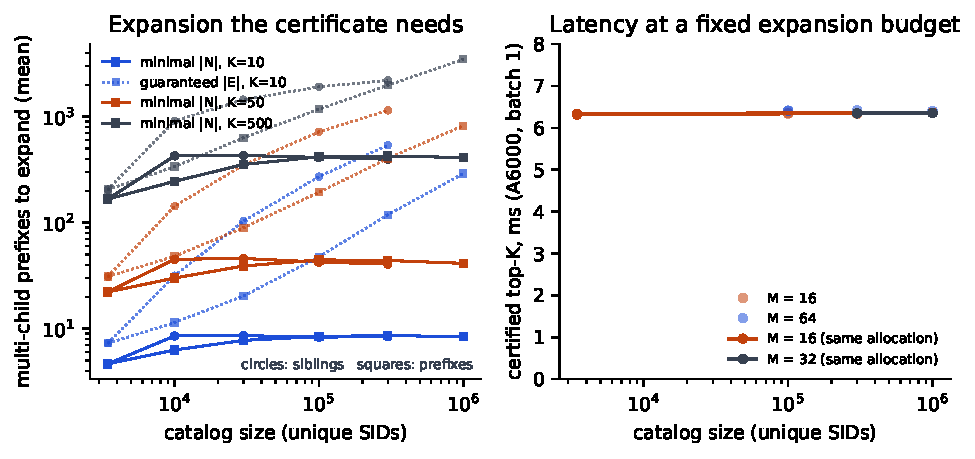
\includegraphics[width=\linewidth]{catalog_scaling.pdf}
\vspace{-6mm}
\caption{Synthetic catalogs of 10k--1M SIDs scored by the real model (500 Office users). Left: the minimal
expansion $|N|$ is flat in catalog size, while the guaranteed set $|E|$ grows with branching. Right: certified
latency at a fixed budget (A6000).}
\label{fig:catalog}
\vspace{-3mm}
\end{figure}

\subsection{RQ4: Late entry}
\label{sec:exp-late}

\begin{table}[t]
\caption{Third-code forward with $k$ of 28 layers, paired against the full-depth forward on all test users
(points; codebook objective). Early exit runs the first $k$ layers; late entry runs the last $k$ (Office: entry
at layer 22; Industrial: 18). Last column: top-1 identical to full depth.}
\label{tab:late}
\vspace{-2mm}
\footnotesize
\setlength{\tabcolsep}{2pt}
\begin{tabular*}{\linewidth}{@{\extracolsep{\fill}}lrrrr@{}}
\toprule
second forward & $k$ & $\Delta$HR@1 & $\Delta$HR@10 & top-1 \\
\midrule
\multicolumn{5}{@{}l}{\emph{Office}} \\
early exit             & 6 & $-3.68\,[-4.34,-3.08]$ & $-0.84\,[-1.29,-0.39]$ & 53\% \\
late entry, ridge      & 6 & $-0.51\,[-0.86,-0.14]$ & $-0.58\,[-1.05,-0.14]$ & 66\% \\
late entry, distilled  & 6 & $+0.27\,[+0.12,+0.45]$ & $-0.04\,[-0.25,+0.16]$ & 94\% \\
\multicolumn{5}{@{}l}{\emph{Industrial}} \\
early exit             & 10 & $-2.38\,[-2.96,-1.83]$ & $-0.77\,[-1.30,-0.20]$ & 47\% \\
late entry, distilled  & 10 & $-0.07\,[-0.22,+0.09]$ & $-0.04\,[-0.24,+0.18]$ & 92\% \\
\bottomrule
\end{tabular*}
\vspace{-3mm}
\end{table}

Table~\ref{tab:late} shows that early exit loses 2.4--3.7 points of HR@1, since the top-1 changes for half of
the users. Late entry with a distilled bridge is statistically indistinguishable from full depth on HR@10 and
NDCG@10 on both datasets. The prefix-weighted KL loss matters: with a uniform loss, HR@1 drops by 0.35 points on
Industrial. With 2 to 14 remaining layers, the distilled bridge stays within $-0.09$ to $+0.14$ points of
full-depth HR@10 (Appendix~\ref{app:extra}). The deployed configuration enters the first code at layer 18 and the third at layer
26. It is lossless against the full-depth model (HR@10 $+0.12\,[-0.27,+0.51]$, NDCG@10 $0.00\,[-0.20,+0.20]$)
and cuts the certified top-10 from 4.35 to 2.75\,ms on an H100. Late entry of the \emph{second} code below layer
18 is a trade-off (NDCG@10 $-0.25\,[-0.51,-0.01]$). That code decides set membership, so we stop at 18. The best
entry layer depends on the model: 26 for the released Office model, 22 after one more fine-tuning epoch, and 18
on Industrial. We choose it on validation.

\subsection{RQ5: Other backbones}
\label{sec:exp-backbones}

\begin{table}[t]
\caption{Other backbones: H100, batch 1, median ms, all test users. The 3B and 7B use Office with the release's
SID index; the SFT/GDPO pair is a 1.5B on Industrial with its own index. Last column: HR@10 with the fused SASRec
term and its gain in points over the same model without it.}
\label{tab:backbones}
\vspace{-2mm}
\footnotesize
\setlength{\tabcolsep}{2.5pt}
\begin{tabular*}{\linewidth}{@{\extracolsep{\fill}}lrrrrr@{}}
\toprule
backbone & beam-50 & certified & + bridge & + SASRec & HR@10 \\
\midrule
1.5B release   & 8.43  & 4.35  & 2.75 & 2.89 & 0.1825 (+1.11) \\
3B (36 layers) & 13.01 & 6.91  & 4.70 & 5.03 & 0.1716 (+2.22) \\
7B             & 21.07 & 11.74 & 7.78 & 8.00 & 0.1683 (+2.38) \\
1.5B SFT       & 5.81  & 4.67  & --   & --   & -- \\
1.5B GDPO (RL) & 5.81  & 5.02  & --   & --   & -- \\
\bottomrule
\end{tabular*}
\vspace{-3mm}
\end{table}

We test public MiniOneRec-format checkpoints that we did not train (Table~\ref{tab:backbones}). Certification
and the 1.8--1.9$\times$ full-depth speedup carry over unchanged to a deeper 3B and a wider 7B model. Certified
top-10 is 99.8--100\% everywhere, and certified decoding matches beam-50 on HR@10 ($+0.12$ and $+0.04$, n.s.).
The third-code bridge, trained with the same recipe, is lossless on both ($-0.06$, $-0.02$, n.s.). It brings the
3B and 7B to 2.8$\times$ and 2.7$\times$ their own beam-50. Fusion helps more when the LLM is weaker: the same
SASRec term adds 2.2--2.4 HR@10 and lifts both above the released 1.5B LLM alone. An RL-tuned (GDPO) checkpoint
makes certification \emph{cheaper}: top-50 certifies at $M=16$ for 26--31\% of users, against 14--20\% for its SFT
parent. RL sharpens the distribution, so fewer prefixes cross the bound.

% =====================================================================================================
\section{Related work}
\label{sec:related}

\paragraph{Serving engines for generative recommendation.} FlashRec~\cite{flashrec} combines wide-beam CUDA
graphs, a fused trie kernel, a per-codebook restricted LM head, radix prefix caching and FP8. NVIDIA's SID-GR
example~\cite{nvidiasidgr} separates shared-context K/V from per-beam K/V with a custom attention kernel.
xGR~\cite{ax2512.11529} separates shared and unshared K/V and filters items with masks. GRACE~\cite{ax2608.00938}
captures the whole SID loop in one CUDA graph. GR4AD~\cite{ax2602.22732} reports gains from beam-shared K/V, a
top-$K$ pre-cut and FP8. STATIC~\cite{ax2602.22647} and FlashTrie~\cite{ax2607.10044} make trie constraints cheap
on accelerators, and UniSGR~\cite{ax2607.04068} uses tree attention over beam candidates. All of these make
beam search faster. We replace it, and our engine reuses the shared-prefix ideas rather than claiming them.

\paragraph{Changing the model.} NEZHA~\cite{ax2511.18793}, SID-MLP~\cite{ax2605.12617} and
Deco~\cite{ax2610.32980} run the LLM once and decode SIDs with a light head. OneRec-V2~\cite{ax2508.20900} and
GR4AD's LazyAR shrink the decoder. GR4AD's LazyAR is the closest in concept to late entry: it \emph{trains} a
decoder whose first layers ignore the previous SID and injects it later. These approaches retrain the model and
are complementary to exact decoding of an unmodified one.

\paragraph{Skipping layers.} Early exit~\cite{schuster2022,elhoushi2024} truncates the top of the network, and
Mixture-of-Depths~\cite{raposo2024} routes tokens around blocks with trained routers. SkipDecode~\cite{delcorro2023}
lets later tokens skip lower layers after fine-tuning, EAGLE~\cite{li2024eagle} drafts features for speculative
decoding, and Hidden Transfer~\cite{ax2404.12022} predicts mid-layer states of unknown future tokens, which must
then be verified. Late entry conditions on the \emph{known} child token and maps across tokens at a fixed depth.
The backbone stays frozen, nothing needs verification, and the result composes with the certificate.

\paragraph{Exact search and scoring.} Exact search in machine translation showed that the MAP output can be worse
than beam search's~\cite{stahlberg2019,meister2020}; exact $n$-best search prunes with the same bound we
use~\cite{stahlberg2022}. In generative recommendation, DiGR~\cite{ax2602.07847} scores every legal SID by brute
force at 5\,s per user, and Yao and Zhu~\cite{ax2611.01072} study where beam search loses top items. Beyond the
Beam~\cite{ax2609.33745} states the same top-$K$ certificate as a post-hoc completion after beam-40 search, with
full-vocabulary scores, certifying top-20 for 4.5--77.6\% of queries. We make it the decoder: every prefix is
bounded in one forward, the expansion set is chosen and, under trie normalization, guaranteed before the second
forward, and 100\% of requests certify. ZeroGR~\cite{ax2611.04715} renormalizes over valid trie children for
speed. We show that this is what makes the bound tight and two-sided. Constrained decoding distorts LLM
distributions~\cite{ax2405.21047,ax2504.09935}. Value-aware decoders~\cite{ax2602.10699,ax2611.02981} mitigate
premature pruning heuristically; certified search handles an additive item value exactly.

% =====================================================================================================
\section{Limitations}
\label{sec:limitations}
We evaluate one model family: MiniOneRec on Qwen2/2.5, from 1.5B to 7B. The real catalogs are small, about
3.5k items with 48--88 first codes, and larger catalogs appear only synthetically. A tokenizer with very wide
first levels (thousands of codes) would need a budget on the first-level expansion as well. Late entry adds a
learned component per model and per entry layer, and the certificate then certifies the bridged objective;
we report quality against the full-depth model throughout. The industry comparison covers one engine, ported by
us, with an unexplained numerical drift. Neither comparison covers long contexts (our prompts are 76--121
tokens; serving engines target 1k--5k) or wide beams ($\ge256$), where shared-K/V designs matter most.

\section{Conclusion}
For LLM generative recommenders with catalog-sized tries, beam search is optional. Two fixed-shape forwards
return the exact top-$K$ of the model's objective with a per-request certificate, and late entry makes the
second forward nearly free. Exactness also makes fusion with item-level terms exact. The result is 2.6\,ms per
request on an H100, 4.5$\times$ faster than a public SID serving engine, and 136$\times$ faster than Hugging Face
decoding on an A6000, with better quality than the model's own beam search.

\bibliographystyle{ACM-Reference-Format}
\bibliography{refs}

% =====================================================================================================
\appendix

\section{Proofs}
\label{app:proofs}
Write $\U(p)=\lp(a)+w_b\lp(b\mid a)$ for $p=(a,b)$. The remaining terms of Eq.~\ref{eq:score} are
log-probabilities scaled by non-negative weights, so $s(i)\le\U(p)$ for every item $i$ under $p$.

\emph{Proposition~\ref{prop:sound}.} Let $s_{(K)}$ be the $K$-th exact score in the pool and suppose
$s_{(K)}\ge\U(p)$ for every unexpanded $p$. Every item outside the pool lies under an unexpanded prefix, so it
scores at most $\U(p)\le s_{(K)}$. No outside item beats the pool's $K$-th item, so the pool's top $K$ is a
global top $K$, up to ties.

\emph{Proposition~\ref{prop:necessary}.} Let $p$ be multi-child and unexpanded with $\U(p)>\tau^*$. A decoder that
has seen only $\U(p)$ cannot rule out a third-code distribution that puts mass $1-\varepsilon$ on one child. That
child scores $\U(p)+w_c\log(1-\varepsilon)$, which exceeds $\tau^*$ for small $\varepsilon$, so it would enter the
top $K$. Hence every such $p$ must be expanded. Best-first expansion by $\U$ expands exactly the prefixes above
the running threshold, which is $N$ up to ties.

\emph{Proposition~\ref{prop:guaranteed}.} Under trie normalization the best child of $p$ has
$\lp(c\mid a,b)\ge-\log n_p$, so some item under $p$ scores at least $L(p)$. Single-child items have exact scores.
The values defining $\tau_L$ therefore each certify a distinct item with score $\ge\tau_L$, so $\tau^*\ge\tau_L$
and $E\supseteq N$. After expanding $E$, the pool contains those $K$ items, so $s_{(K)}\ge\tau_L$, and every
unexpanded prefix has $\U<\tau_L\le s_{(K)}$. Proposition~\ref{prop:sound} applies. $E\setminus N$ contains only
prefixes with $\tau_L\le\U<\tau^*$, a band of width at most $w_c\log n_{\max}$.

\section{Engine and latency ladder}
\label{app:engine}

\begin{table}[h]
\caption{Latency ladder, Office, batch 1, median ms. The A6000 rows come from one allocation, as do the H100
rows; the final rows are from a later allocation.}
\label{tab:ladder}
\vspace{-2mm}
\small
\setlength{\tabcolsep}{3pt}
\begin{tabular*}{\linewidth}{@{\extracolsep{\fill}}lrr@{}}
\toprule
step & A6000 & H100 \\
\midrule
Hugging Face \texttt{generate}, FP32                 & 868.8 & -- \\
our engine, FP32, beam-50                            & 100.8 & 48.3 \\
BF16, one CUDA graph per request                     & 42.1  & 20.1 \\
+ \texttt{torch.compile}                             & 35.0  & 12.9 \\
+ first trie level fused into the prompt forward     & 28.1  & 8.50 \\
+ FP16, cached prompt template                       & 26.2  & 8.48 \\
certified exact decoding (trie)                      & 14.4  & 5.57 \\
+ multi-child prefixes only, Triton prompt attention & 13.25 & 4.37 \\
+ late entry, third code at layer 22                 & 8.98  & 3.32 \\
+ first level at 18, third code at 26 (final)        & 6.38  & 2.75 \\
+ SASRec term (in the graph on the H100)             & 6.44  & 2.89 \\
\bottomrule
\end{tabular*}
\end{table}

FP16 with a pre-scaled query matches FP32's top-1 for 500/500 cohort users; BF16 matches for 488/500. On the H100
the engine is bound by kernel count, not bandwidth. The first certified decoder issued 2,555 kernels and spent
5.9\,ms of GPU time per request. Late entry and a Triton prompt attention cut this to 1,474 kernels and 3.7\,ms.
Fusing the forced suffix into one two-token forward saves 10\,ms on the A6000 for the beam baselines.

\section{What exact decoding reveals about the objective}
\label{app:objective}

\begin{table}[h]
\caption{Scoring rules under beam-50, Office, all test users.}
\label{tab:scoring}
\vspace{-2mm}
\footnotesize
\setlength{\tabcolsep}{3pt}
\begin{tabular*}{\linewidth}{@{\extracolsep{\fill}}lrrrr@{}}
\toprule
scoring rule & HR@1 & HR@10 & NDCG@10 & HR@50 \\
\midrule
full vocabulary + suffix (MiniOneRec) & 0.0947 & 0.1589 & 0.1249 & 0.2370 \\
full vocabulary, no suffix            & 0.0986 & 0.1624 & 0.1284 & 0.2363 \\
trie                                  & 0.0982 & 0.1648 & 0.1287 & 0.2417 \\
codebook (FlashRec)                   & 0.0986 & 0.1667 & 0.1299 & 0.2470 \\
\bottomrule
\end{tabular*}
\end{table}

\paragraph{Beam search error grows with list length.} From exhaustive FP32 scores of every SID for every user,
beam-$W$ under the full objective recovers 49\%, 53\% and 64\% of the exact top-$W$ for $W=50$, 100 and 500
(Industrial: 67/69/79\%). Under trie scoring it recovers 95/96/99.6\%. Under the full objective, exact search
\emph{loses} recall at large $K$ (HR@500 $-4.3\,[-5.3,-3.2]$ vs.\ beam-500). Under the validation-tuned codebook
objective it \emph{gains} recall (HR@500 $+2.4\,[+1.4,+3.3]$). Beam search's prefix-first pruning acts as an
implicit depth discount; once the discount is explicit, exactness stops hurting.

\paragraph{Why the deep terms mislead.} Over 1,217 Office users $\times$ 3,444 SIDs:
(i) \emph{Sibling penalty}: $\lp(c\mid a,b)$ falls with the number of catalog items sharing $(a,b)$, with median
$-0.87$, $-2.46$, $-3.05$, $-3.38$ and $-4.12$ for 1, 2, 3, 4 and 6 siblings. That is steeper than an even split,
a structural penalty unrelated to the user (Fig.~\ref{fig:sibling}).
(ii) \emph{Codebook leakage}: even after a valid $(a,b)$, a median 47\% of next-token mass falls outside the
$c$-codebook, which full normalization charges unevenly.
(iii) The forced suffix acts as a weak popularity prior ($r=0.15$ with log popularity). It moves the target up
for 28\% of users and down for 25\%.

\begin{figure}[h]
\centering
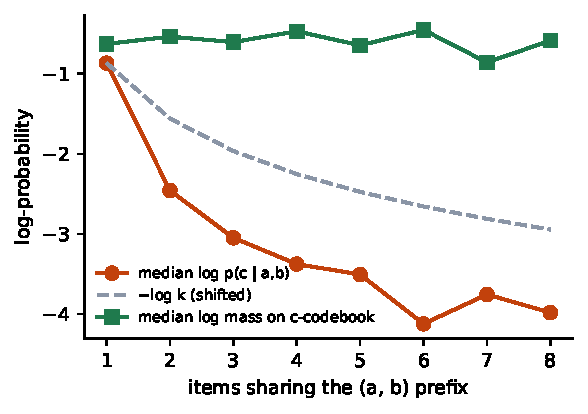
\includegraphics[width=0.8\linewidth]{sibling_penalty_office.pdf}
\vspace{-3mm}
\caption{The sibling penalty (Office, exhaustive FP32 scores).}
\label{fig:sibling}
\end{figure}

\section{FlashRec comparison details}
\label{app:flashrec}
We use FlashRec 0.1.2 (commit 1089682, Apache-2.0). Our patch adds Qwen2's QKV bias and removes QK-norm. When
there is no norm, it runs FlashRec's fused RoPE + FP8 K/V-store Triton kernel with the normalization disabled.
FlashRec's CUDA graphs are captured at 19 sizes, and its JIT trie kernel is verified loaded. Latency is the wall
time of \texttt{engine.generate()} from token ids to ranked beams on the host. Ours is a pinned host prompt through
one graph replay; copying the list back to the host adds 0.02\,ms.

\emph{Numerical drift.} On our port, FlashRec's first-code log-probabilities differ from Hugging Face FP32 by 0.23
nats on average. Hugging Face in half precision differs by 0.002 (FP16) and 0.02 (BF16). FlashRec's top-1 agrees
with exact beam under the same objective for 80\% of users. The drift persists when we disable each component we
could isolate: the radix cache, CUDA graphs, fused expansion, the per-codebook head, GQA grouping (a
12-KV-head copy drifts the same), output-layer tying, Q/K layout, and its pre-cut of $2\times$beam candidates.
We report FlashRec as measured and also our exact implementation of its objective. Speed is unaffected, since
the computation is the same.

\section{Additional results and negative results}
\label{app:extra}
\emph{Late-entry depth.} With a uniform-KL bridge on Office, keeping 2/4/10/14 layers gives HR@10 deltas of
$-0.09/+0.04/\text{n/a}/+0.14$ and HR@1 deltas of $-0.45/-0.27/+0.06/-0.02$; top-1 agrees with full depth for 86--94\% of
users.
\emph{One forward is not enough.} A user-independent table of third-code scores keeps HR@10 within 0.9 points
but halves HR@1 (0.098 $\to$ 0.050). Guessing the expansion set before Forward~1, from history or popularity,
covers the certificate set for top-10 in at most 29\% of requests.
\emph{Quantization.} Weight-only INT8 is quality-neutral but only 3--8\% faster, and INT4 is no faster. At
50--216 rows per forward, GEMMs are past the regime where weight-only kernels help. Static FP8 is slower than
BF16 on an L40S. Dynamic per-token FP8 on the H100 is quality-neutral and adds 16--21\% throughput.
\emph{Training for the decoder.} One more SFT epoch with a loss aligned to the decoder's restricted normalization
improves HR@10 by $+0.90\,[+0.27,+1.54]$ over the release. A full-vocabulary control gets almost all of it
(aligned vs.\ control $+0.14\,[-0.16,+0.47]$), so the alignment itself does not help.

\section{Reproducibility}
\label{app:repro}
Code, the FlashRec patch and every run are in the repository (anonymized for review). Bridges train on the
validation split only; weights and $\beta$ are chosen on validation and evaluated once on test. Hardware: NVIDIA
H100 80GB and RTX A6000 (L40S and A40 for FP8 and catalog-scaling runs). Main runs: \texttt{runs/frLat},
\texttt{frTp} (Table~\ref{tab:speed}); \texttt{finalH}, \texttt{collabO}, \texttt{fuseI} (Table~\ref{tab:quality});
\texttt{lbndA} (Table~\ref{tab:bounds}); \texttt{scaleP}, \texttt{scaleI} (Fig.~\ref{fig:catalog});
\texttt{ladder2}, \texttt{h100M} (Table~\ref{tab:ladder}).

\end{document}
